
\section{Model comparison with measurements: anomalous heating in the edge.}\label{sec:results_results}
\begin{figure}
    \centering
    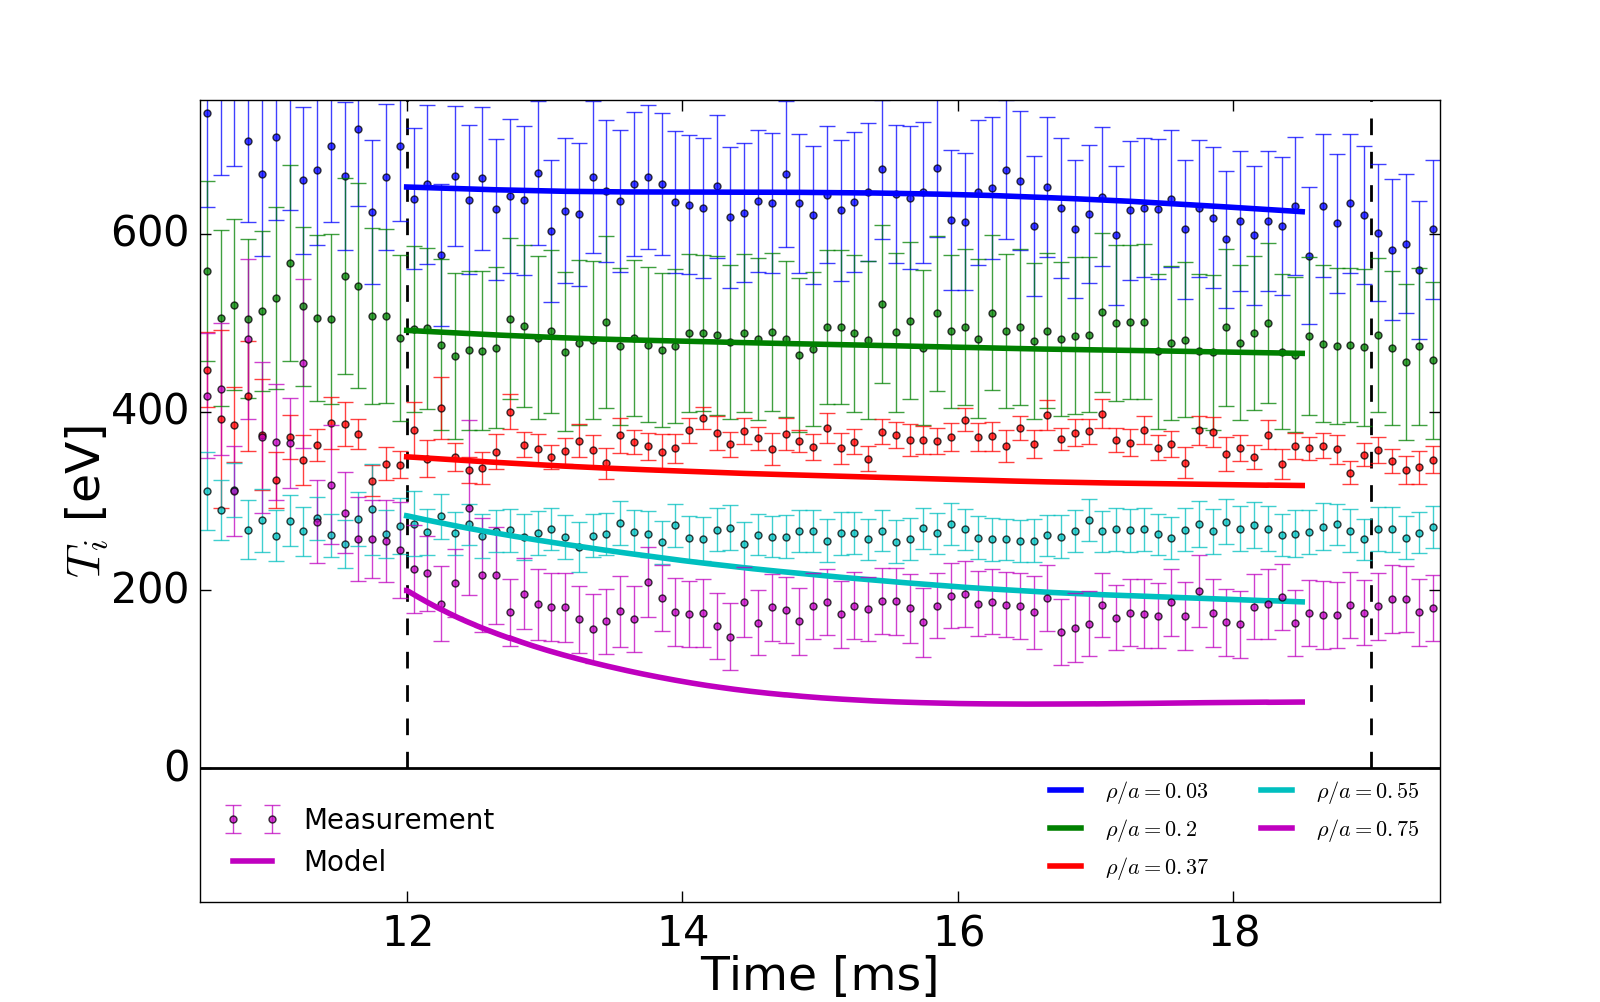
\includegraphics[width = \linewidth]{ion_transport_results/temperature_results.png}
    \caption[Temperature comparison with measurement]{Temperature comparison with measurement.}
    \label{fig:temperature_results}
\end{figure}

\begin{figure}
    \centering
    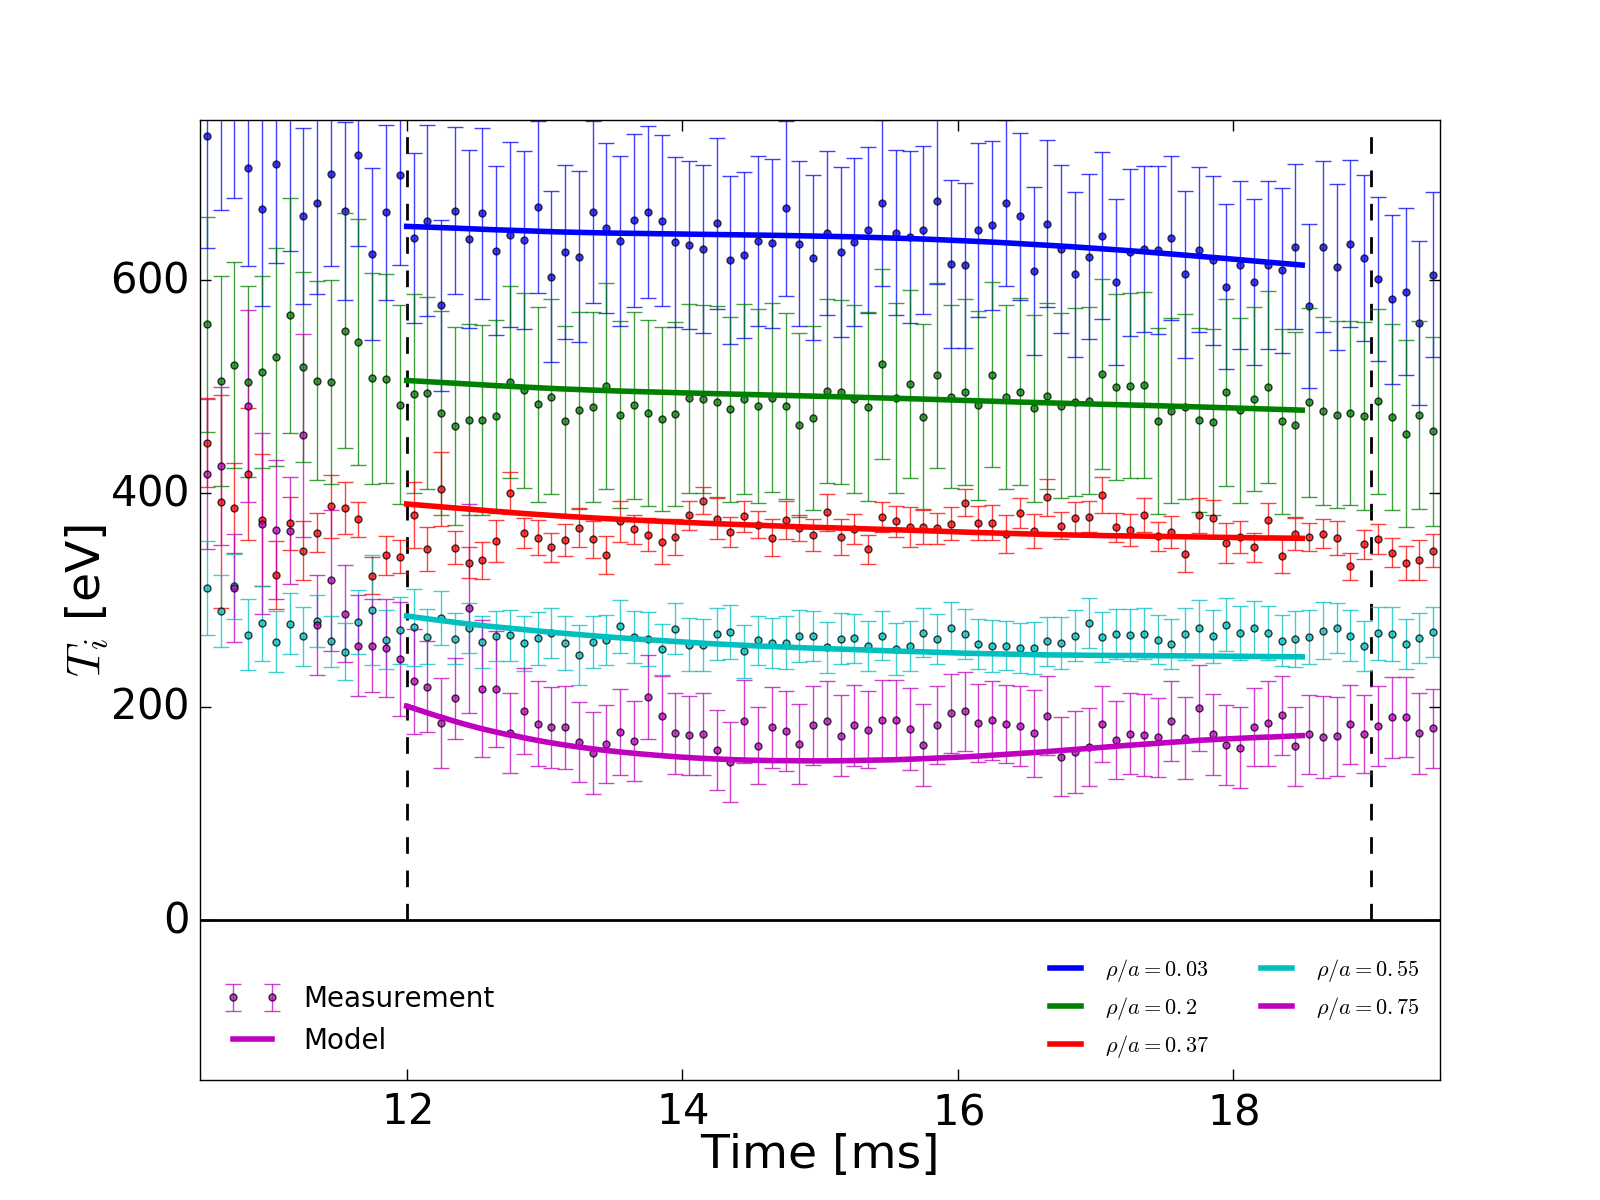
\includegraphics[width = \linewidth]{ion_transport_results/temperature_with_adhoc.png}
    \caption[Temperature comparison with measurement with \textit{ad hoc} term included]{Temperature comparison with measurement with \textit{ad hoc} term included.}
    \label{fig:temperature_results_ah}
\end{figure}

\begin{figure}
    \centering
    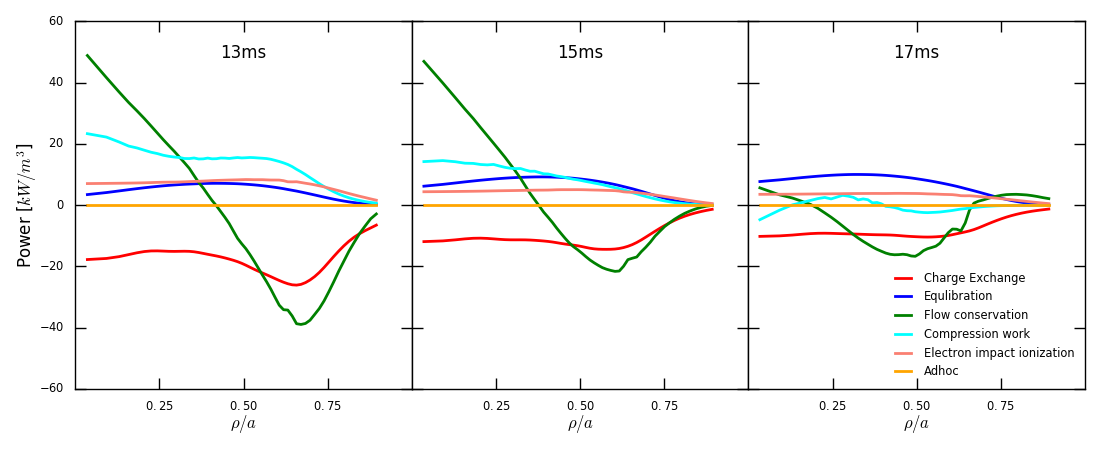
\includegraphics[width = \textwidth]{ion_transport_results/power_terms_no_adhoc.png}
    \caption[Power terms resulting from radial ion flow]{Power terms resulting from radial ion flow.}
    \label{fig:power_terms_no_ahoc}
\end{figure}
The quality of the model is evaluated by comparing its prediction to the ion temperature measurement made with CHERS. The model is initiated at 12ms, about 2ms after the first PPCD capacitor bank 'fires', as it is the earliest time when the significant suppression of tearing mode turbulence are achieved. CHERS measurement of temperature at initialization time is fit to an alpha model profile and then input into the model as initial condition. The time evolution of ion temperature is calculated according to the physics terms described in the previous sections and chapters. The model is found to adequately predict the temperature in the core, but not in the edge. To account for the edge temperature, an \textit{ad hoc} heating term is added. The model comparison results can been seen in figure \ref{fig:temperature_results}.  The most significant power loss terms (figure \ref{fig:power_terms_no_ahoc}) affecting this region is charge exchange, and thermal energy carried by particle flow (flow conservation). It is interesting to note that these loss terms are to a large extent a function of temperature as much if not more than as a function of temperature gradient. This dependence on $T_i$ is a factor that result in there being an 'equilibrium' temperature for the model. For the case where no \textit{ad hoc} heating is included, the ion temperature at near the edge would decrease until it levels off at significantly lower temperatures than the measured. In particular, figure \ref{fig:temperature_results} superficially suggest that (for the edge chord location) the temperature decreases rapidly early during the PPCD period. But initializing the model at later starting time would have the model reproduce the same behavior and settle at the same edge temperature, just now delayed. This indicates that it is not some particular circumstance relating to the early PPCD period that causes the model to under predict the temperature. But the model behaves in such a way that the edge temperature trends towards and `equilibrium' temperature determined by the power terms, which is significantly lower than the actual equilibrium temperature that the ion fluid comes to. To remedy this under prediction, an \textit{ad hoc} term is introduced into the model to raise the model's 'equilibrium'. The particular profile shape and location used for the \textit{ad hoc} term is discussed in detail in the next section, but the result of this are presented in figure \ref{fig:temperature_results} and \ref{fig:power_terms_with_adhoc}. With this addition, the model is able to account for the temperatures measured by CHERS. In this scenario, the core power terms are dominated by the effects of flow, in particular compressional heating and flow conservation. It is also useful to refer to figure \ref{fig:temperature_change} which provides information on how each term effects $T_i$. From this figure it is easier to see the importance of the compressional heating term on the core temperature prediction. $P_{\text{comp work}}$ is the larger of only two terms increasing temperature in the core, and is a major part of how the model matches a flat-ish fore $T_i$ evolution observed. Towards the edge, the major heating (thermal energy input) term is the \text{ad hoc} term. $P_{\text{flow cons}}$ is negative in the edge and the most significant source of loss. One looking at $\partialt T_i$ plot would come to the (almost) paradoxical conclusion the the flow conservation term is significant in maintaining temperature. This can be understood by pointing out the outward particle flow in the edge have the net effect of removing a number of ions at the local temperature, and replacing them with a smaller number of hotter ions from inner flux surfaces, thus increasing temperature. The density balance is achieved though a large ionization source rate, which reduces $T_i$ despite bringing some thermal energy with it (due to non-zero neutral temperature).


\begin{figure}
    \centering
    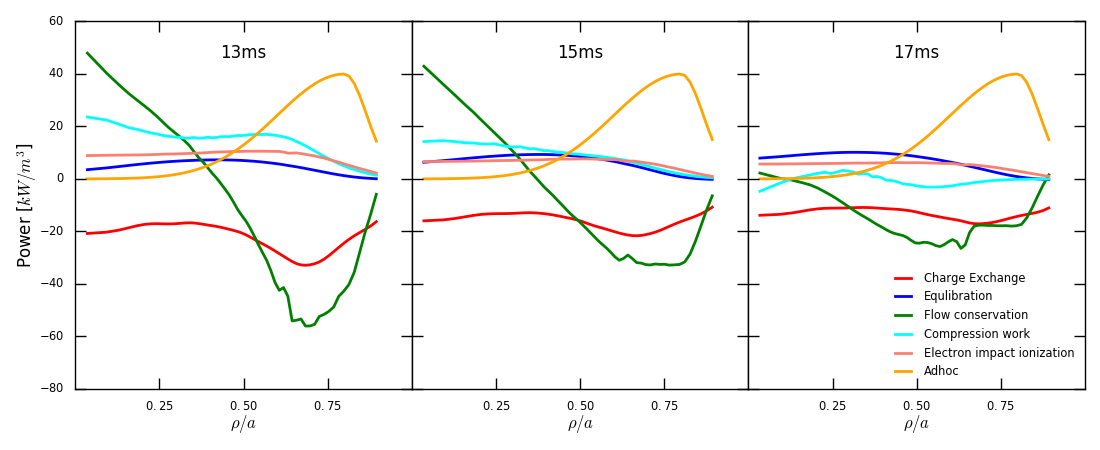
\includegraphics[width = \textwidth]{ion_transport_results/power_terms_with_adhoc.png}
    \caption[Power terms resulting from radial ion flow]{Power terms resulting from radial ion flow. Classical conduction have been omitted as it is of lower magnitudes than the plotted terms.}
    \label{fig:power_terms_with_adhoc}
\end{figure}


%TODO: There should be a paragraph on estimating the ion thermal confinement time that I'm not quite ready to write yet. 

From this model, the ion thermal confinement time can be estimated. The common definition of thermal confinement time is written as follows,
\begin{align}
    \tau_E &= \frac{W}{P_{\text{loss}}}\\
    &= \frac{W}{\partialt W - P_{\text{ohm}}}
\end{align}
However, in the context of the model, where the loss terms are known explicitly, it is more appropriate to specify $P_{\text{loss}}$ directly. In particular, 
\begin{align}
    P_{\text{loss}} &= - [P_{\text{CX}} + P_{\text{cond}} + P_{\text{flow cons}}]
\end{align}
The other terms in the model, including compressional work, \adhoc heating, and e-i equilibration heating, are considered power inputs, and thus do not factor into the calculation of the thermal confinement time. 
 % I don't think that these terms are 'external' to the plasma the way Ohmic heating or RF heating are external inputs to the plasma. By they are power inputs to the ion fluid rather than losses.
 %Edited -Xing
This means that for the consideration of this calculation, the flow terms as specified in section \ref{sec:flow_effects} are separated into the compressional heating part ($P_{\text{comp work}}$) which is not part of $P_{\text{loss}}$, and the flow conservation part ($P_{\text{flow cons}}$) which is. The confinement time of the model is shown in figure \ref{fig:conf_time}. It should be noted that this is not a direct measurement of the ion confinement time, but rather it is the ion confinement of a model that can be matched to observed temperature evolution.
\begin{figure}
    \centering
    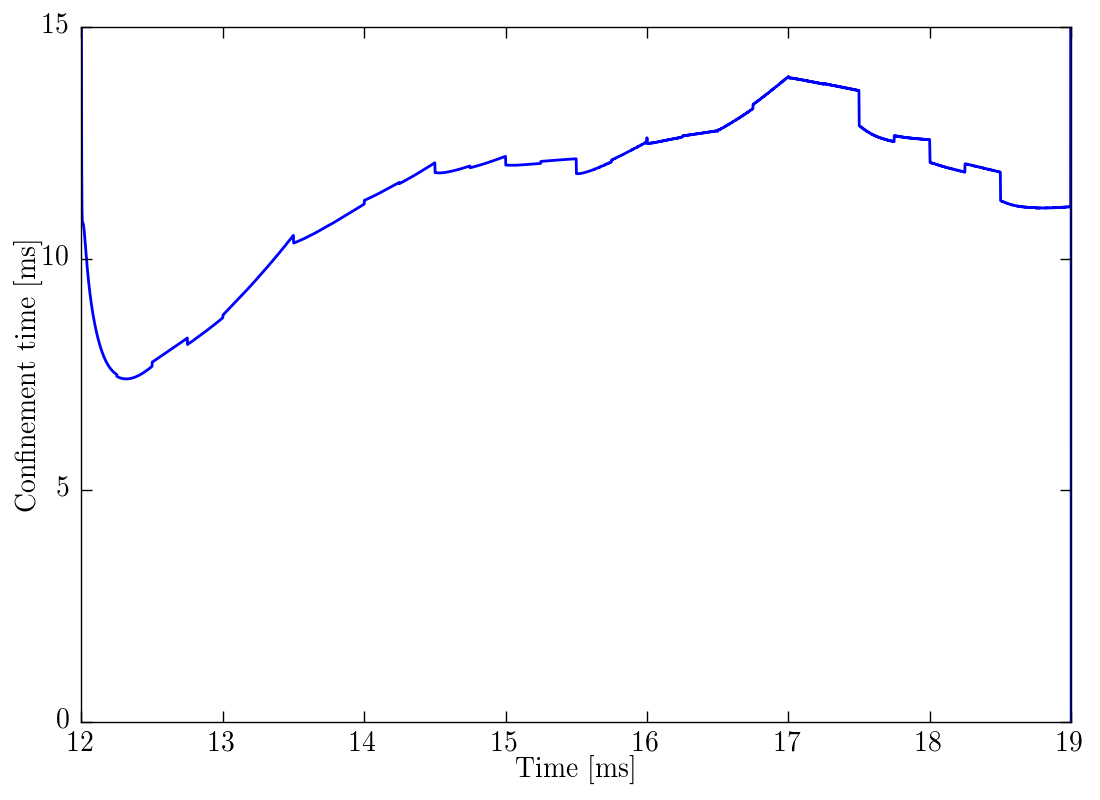
\includegraphics[width = \linewidth]{ion_transport_results/conf_time.png}
    \caption[Model ion confinement time]{Ion confinement of the model. It is calculated to be around 12ms for the 'main' part of PPCD (~15ms to the end of PPCD). The confinement time is poorer during onset of PPCD (< 15ms) but displays a roughly upward trend. The effect on temperature of this relatively poorer confinement is mitigated by the compressional heating active during the early period. }
    \label{fig:conf_time}
\end{figure}
The thermal confinement time is comparable to electron confinement time in PPCD calculated at ~ 10ms \cite{Chapman2001}, but it is not evident that the two are linked through physical mechanisms. Considering the decoupling of ion and electron temperature, it may be a coincidence that their confinement time seems to match. The model's confinement time further changes if the model temperatures are allowed to drift below the observed temperature by omitting the \adhoc heating term. In that case, the confinement time noticeably increase as the edge ion temperature decreases which decreases the heat loss due to outward particle flux in the edge, as well as somewhat reducing the charge exchange loss the the same region. 
%%% Now that you have calculated the ion thermal confinement time, how does it compare with other relevant time scales? For instance, how does it compare with the electron thermal confinement time for PPCD or standard plasmas? Are the results what you would expect or are they surprising?
%Elaborated. --Xing

\subsection{Profile and extent of \adhoc heating in the gradient regions}\label{sec:anomalous_heating}

The previous section glossed over the shape and location of the \textit{ad hoc} heating term used in order to present the results. However, there are comments to be made that would be of interest to readers. The driving determinant of the \textit{ad hoc} term is to enable the model to match the observations, but that does not mean that it is entirely free of physics considerations. The profile settled upon is an asymmetrical Gaussian (in $\rho_v$) made from two half Gaussian profiles with differing width. The profile peaks at $\rho_v/a = 0.75$, the approximate location of the reversal surface (see figure \ref{fig:q_profile}). The reversal surface is not only the home of all m = 0 modes, but also near tightly packed m =1 rational surfaces. Additionally, the peak and the width of the \textit{ad hoc} heating term is approximately coincident with the $T_e$ gradient region as measured via Thomson scattering. The edge half of the Gaussian shape have a smaller width to account for the fact that the turbulence that likely drives anomalous heating would be rapidly decreasing near MST's conducting shell, together with rapidly decreasing availability of free energy as temperature and density drops in the very edge. However, the modeling work and the CHERS measurements provide nearly no constraint on the very edge of the plasma. 
\begin{figure}
    \centering
    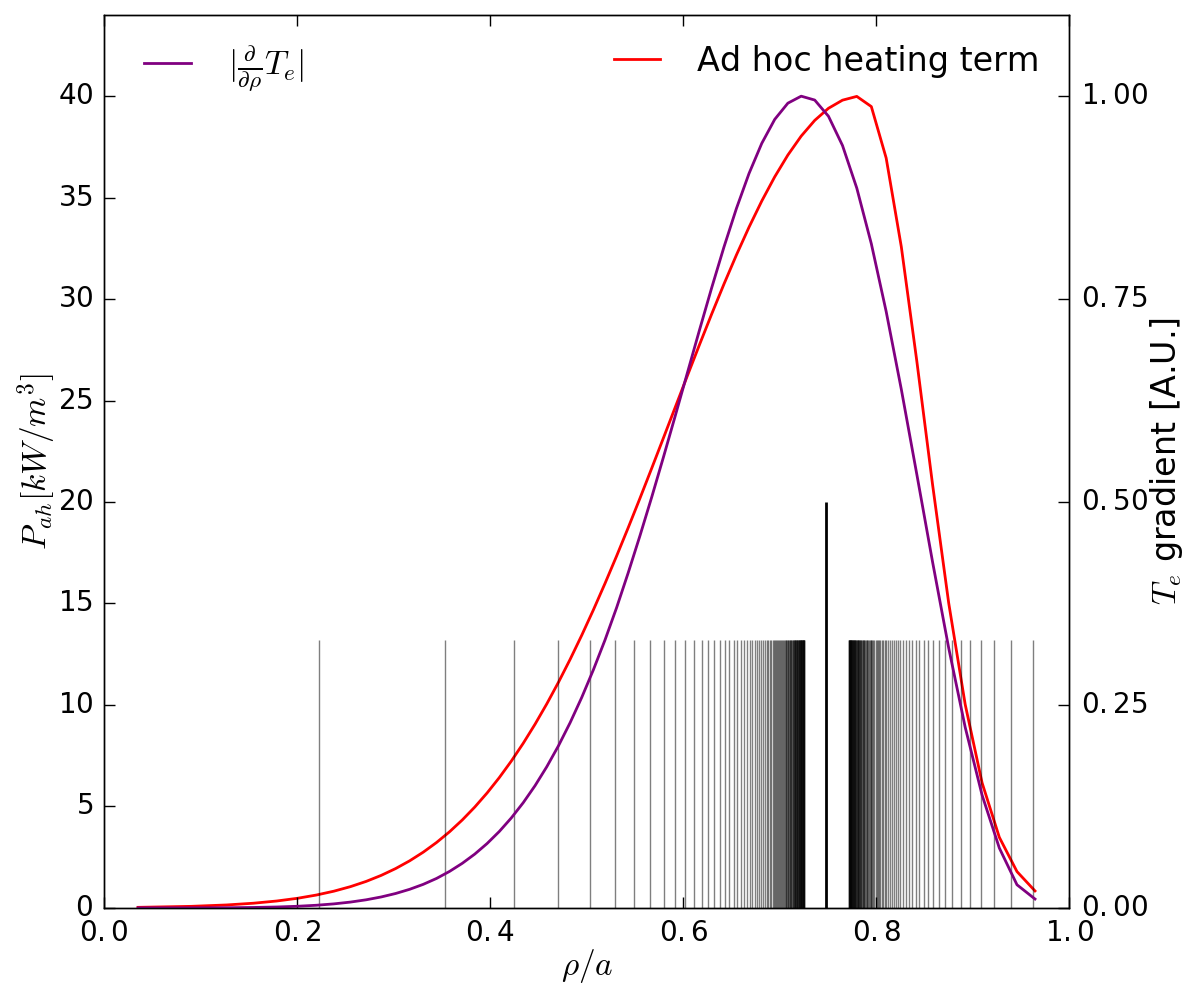
\includegraphics[width = \textwidth]{ion_transport_results/adhoc_profile.png}
    \caption[\textit{ad hoc} heating profile]{\textit{ad hoc} heating profile compared to normalized $T_e$  gradient. The long vertical line at $\rho/a \approx 0.75$ marks the location of the reversal surface, and the shorter lines marks out the resonant surfaces beginning with inner most the (1,6) surface. For a plot of the q profile associated, see figure \ref{fig:q_profile}.}
    \label{fig:ad_hoc_v_gradient}
\end{figure}
%Mark comments here:
%In addition to mentioning the edge localization, you should note that there are several sources of free energy that could drive heating mechanisms. First, there is residual tearing mode activity in PPCD plasmas that, while much lower in amplitude, still result in stochasticization of the magnetic field near the reversal surface. In addition, we are actively driving a current in the edge and may be affecting the current gradient in such a way that it can excite the edge-resonant modes. Finally, there is the edge density gradient which drives drift wave instabilities that give rise to turbulent electrostatic fluctuations.

%These are all free sources of energy that could provide sufficient energy for the modest amount of edge-localized ion heating your model suggests. This energy could be tapped through processes like turbulent damping of Alfven-waves through cyclotron resonance, stochastic heating due to the residual tearing modes near the reversal surface, driving edge-resonant tearing through the PPCD pulses, and turbulent heating which can channel heat from the electrons to the ions.
 
%For the last process, I started with Gennady’s paper and potentially made a mistake. For Gennady’s argument to be self-consistent the perpendicular diffusion process has to be separate from the process generating the electric field fluctuations. Otherwise, there is a problem with making the process irreversible.

%A more natural way of formulating the heating mechanisms available through drift wave turbulence is to consider ion Landau damping and frictional heating associated with zonal flow generation by the turbulence. A paper which lays these mechanisms out is here:
There are several mechanisms that may be responsible for this \adhoc heating, including cyclotron resonance heating from Alfven waves and stochastic heating from residual tearing modes activities near the reversal surface. Further, plasma turbulence such as driftwaves and zonal flow, both recently observed for PPCDs in MST\cite{Nishizawa2018, Nishizawa2019}, drives both quisilinear and nonlinear turbulent heating and enables the collisionless transfer of energy from electrons to ions through such mechanisms such as Landau damping of wave energy, and frictional heating via zonal flow. The volume integrated \adhoc heating used in the model is $\approx 144 kW$, which is small in the overall energy balance of the RFP. For example, the total magnetic energy ($ = \frac{B^2}{2\mu_0}$) goes from $\approx 275kJ$ to $\approx 300kJ$ and back during a typical period of analysis (spans 8ms from 12ms to 20ms). Thus a seemingly small transfer of energy from electrons or the magnetic equilibrium may be sufficient to account for the \adhoc heating added to model calculations.

More generally, the location and the width of the \textit{ad hoc} heating term roughly corresponds with the location of the $T_e$ gradient region (see figure \ref{fig:ad_hoc_v_gradient}). While electron gradients are not directly connected to ion thermal heating, they are sources of free energy driving turbulence that would generate heating. 

\subsection{Anomalous Transport vs. heating}

The \textit{ad hoc} heating term needed for the model can correspond to anomalous transport or heating, as the model does not account for stochastic transport mechanisms, or turbulent heating mechanisms. However, given the model's ability to predict the core temperature well even in the absence of the \textit{ad hoc} term, it is more likely that the discrepancy in the edge is accounted for by anomalous heating. 
Consider stochastic transport of heat, the stochastic counterpart to classical thermal conduction. The stochasticity increases the characteristic step size of the particle beyond the gyro-radius, and ions wondering along the stochastic field would collide another and exchange place' with it, transporting heat from the hotter location to the colder. Note that this is a purpose effort to separate the stochastic heat conduction/transport from the stochastic particle transport, as the particle transport and flux is indirectly included in the model (see the discussion in section \ref{sec:stochastic_effects}). The total \adhoc term needed in the model integrates to about 140kW over the volume of the plasma. If the \adhoc term is 'caused' by a anomalous transport mechanism, then the transport mechanism would be taking the thermal energy from hotter regions (\textit{ie.} core). For an estimation, one can assume that such a transport mechanism takes heat from the core region defined by $\rho/a \leq 0.4$ and deposit at $0.4 \leq \rho/a \leq 0.9$ (refer to figure \ref{fig:ad_hoc_v_gradient}). Thus defined, the core region have a volume of $\approx 1.25 m^2$, and lose heat at $~110kW/m^2$ making it the most significant term in the core. Further assuming a nominal core density of $0.7 \times 10^{19}/m^3$, the core cooling implied by such a transport would be $\approx 100eV/ms$ in addition to what the model currently predicts. This is significantly larger core cooling than the observations would allow (refer to figure \ref{fig:temperature_results_ah}).

While it cannot be ruled out that the \adhoc term in the model is the result of a combination of a anomalous transport mechanism, and a (relatively) radially uniform anomalous heating mechanism, it is very unlikely to be the effect of a anomalous transport mechanism only. To the first order, the result point to an anomalous heating mechanism active in the $T_e$ gradient region.

\subsection{Additional comments on thermal transport}

\begin{figure}
    \centering
    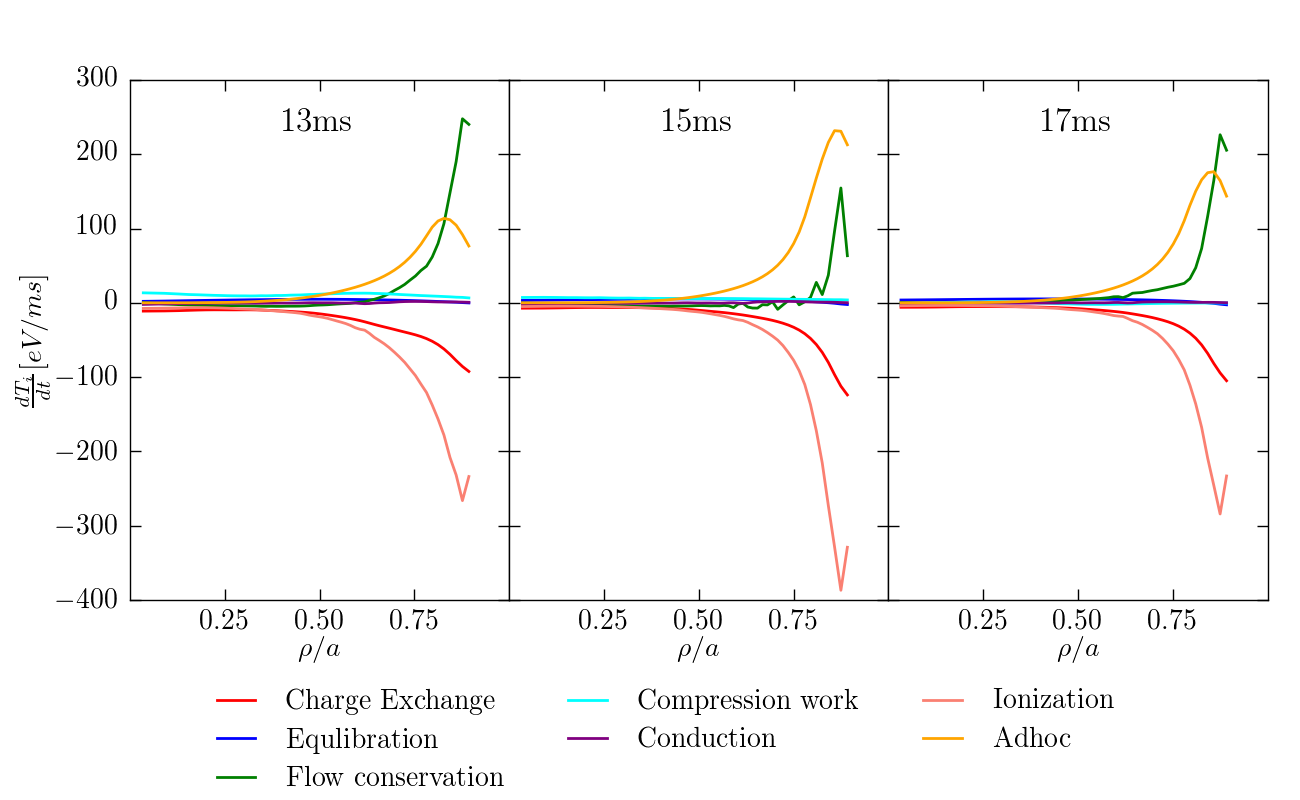
\includegraphics[width = \linewidth]{ion_transport_results/dtempdt_with_adhoc.png}
    \caption[$\partialt T_i$ due to various terms]{$\partialt T_i$ due to various terms in the model. The significance of this plot is explored more in the text. }
    \label{fig:temperature_change}
\end{figure}

\begin{figure}
    \centering
    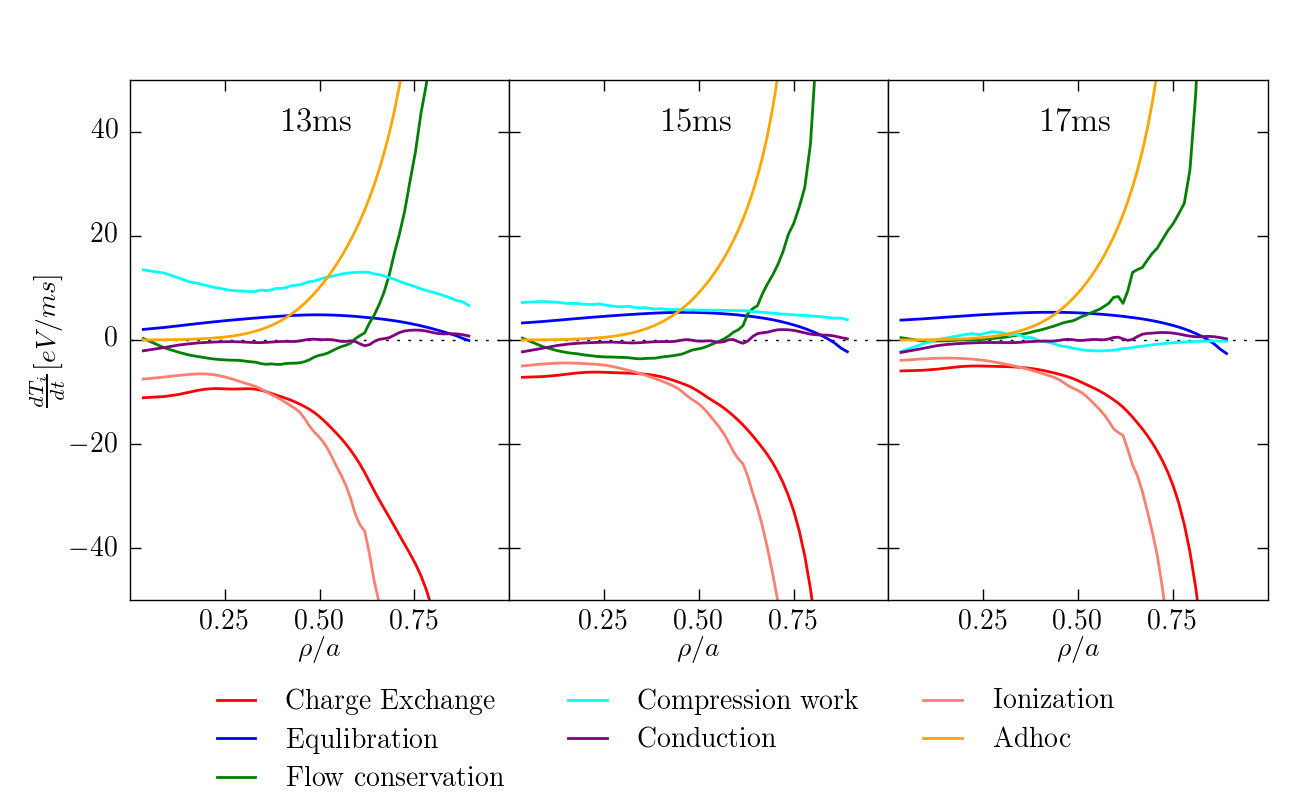
\includegraphics[width = \linewidth]{ion_transport_results/dtempdt_zoomed.png}
    \caption[$\partialt T_i$ core details]{$\partialt T_i$ due to various terms in the model, zoomed in to show the core dynamics clearer. Note the disappearing effect of compressional work. }
    \label{fig:temperature_change_zoomed}
\end{figure}

It is instructive to look at the modeled terms from the point of view of their contribution to $\partial T_i /\partial t$ (figure \ref{fig:temperature_change} and figure \ref{fig:temperature_change_zoomed}). There is two effects worth noting. The first is that some power terms do not have the same effect on temperature as thermal energy. As mentioned before, $P_{\textrm{ionization}}$ which represents the energy 'recovered' from the warm neutral population through re-ionization, reduces the ion temperature despite being a positive power term. This is due to the fact that it brings cooler particles into to the ion fluid. The cooling effect of ionization is the most significant in the edge region, but important throughout the plasma volume. Conversely, the flow effects are (aside from the \textit{ad hoc} term) the most significant for increasing the temperature, due to the flow of hotter ions to the cooler edge. But at the same time, it competes with charge exchange for being the significant energy loss term. The second is that the $P_{\textit{ad hoc}}$ contribution to $\partial T_i / \partial t$ is modified by density, causing it to chage despite the power remaining constant. Especially, it's peak is farther out in the edge as compared to that of $P_{\textit{ad hoc}}$ itself. Looking at figure \ref{fig:temperature_change_zoomed}, we can see that \textit{ad hoc} term's contribution to $\partial T/\partial t$ is relatively constant inside $\rho/a = 0.75$. The response outside of this location (\textit{i.e.} the outside half-Gaussian of the \textit{ad hoc} profile) changes significantly. Though the model is not well constrained here, as the outer most CHERS measurement is at $\rho/a = 0.75$. If the \textit{ad hoc} heating is indeed related to the stochastic mechanism as detailed by G. Fiksel, the $\left.\partial T_{i}/\partial t\right|_{\textit{ad hoc}}$ would be relatively constant and the resultant power would change as density changed. 

The e-i equilibration term is generally weak, resulting in the temperature separation seen in PPCD plasmas. Extrapolating to typical reactor densities, however, would imply that the equilibration heating would in crease by ~ 2 order of magnitude (both $n_e$ and $n_i$ would increase by an order of magnitude) while the biggest core loss term, charge exchange, would increase less as the neutral sourcing will increase will plasma density, but the neutral penetration will decrease correspondingly. As is currently, the charge exchange loss and the net flow loss (aka particle loss) are the two main loss mechanisms. Efforts to limit neutrals in the plasma may be beneficial, but high density and temperature plasmas, the neutrals are likely to have a much reduced role. Net ion particle loss will likely be the dominant challenge to RFP ion confinement in PPCD-like conditions. 

